\section{Models}
Two different models were developed for the sentiment analysis task. The first model is a Recurrent Neural Network (RNN) with Long Short-Term Memory (LSTM) cells, and the second model is a Transformer model.

\subsection{Model 1: RNN-LSTM}
\subsubsection{Model Architecture}
We chose to begin with a Recurrent Neural Network (RNN) model using LSTM (Long Short-Term Memory) cells due to their proven effectiveness in capturing long-term dependencies in sequential data, such as text. LSTMs are particularly suited for this task because they address the vanishing gradient problem often encountered in standard RNNs.

The architecture of the model was designed to balance complexity and performance, resulting in a total of 1,117,734 trainable parameters. Key considerations behind the design are as follows:
\begin{itemize}
    \item Embedding Layer: The vocabulary size of 10,336 and embedding dimension of 75 were chosen to compactly represent the input text while capturing semantic relationships between words effectively. This dimensionality ensures the embeddings are rich enough for the sentiment classification task without being computationally excessive.
    \item LSTM Layer: A single LSTM layer with 256 hidden units was selected to provide sufficient capacity to capture sequential patterns in the text. This configuration was chosen to avoid overfitting while retaining the ability to model complex dependencies in the data.
    \item Dropout Layer: A dropout rate of 50\% was applied to the LSTM outputs to reduce the risk of overfitting by preventing the model from becoming overly reliant on specific neurons. This regularization technique ensures better generalization to unseen data.
    \item Output Layer: The final linear layer maps the 256 features to the 6 output classes, corresponding to the emotions in the dataset.
\end{itemize}

The specific parameters mentioned above was found using a combination of empirical testing (grid search) and theoretical considerations to achieve a balance between model complexity and performance.

\subsubsection{Training and Evaluation}
The model training was conducted using the AdamW optimizer with a learning rate of 0.001 and a batch size of 16. AdamW was chosen due to its effectiveness in handling sparse gradients and its built-in weight decay mechanism, which helps prevent overfitting. The batch size of 16 strikes a balance between computational efficiency and the stability of gradient updates.

For the loss function, we used CrossEntropyLoss, which is well-suited for multi-class classification problems like this one, where the task involves predicting one of six emotion categories. To further regularize the model and reduce the risk of overfitting, an L2-norm penalty (weight decay) of 0.0001 was applied to the weights, encouraging smaller parameter values and promoting a simpler model. The model was trained for 4 epochs, as using more epochs lead to overfitting. The final test accuracy and F1-score is summarized in Table \ref{tab:rnn_lstm_model_test}.
\begin{figure}[H]
    \vspace*{0.7cm}
    \centering
    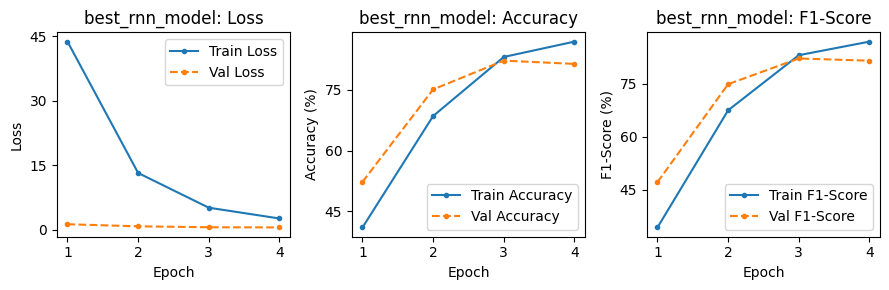
\includegraphics[width=0.6\textwidth]{figures/rnn_scores.png}
    \caption{Training and validation loss, accuracy, and F1-score for the RNN-LSTM model.}
    \label{fig:rnn_scores}
    \vspace*{0.7cm}
\end{figure}

\begin{table}[H]
    \vspace*{-0.5cm}
    \centering
    \begin{tabular}{|l|c|c|c|}
        \hline
        Label        & Precision & Recall & F1-Score \\ \hline
        sadness      & 0.91      & 0.86   & 0.89     \\ \hline
        joy          & 0.85      & 0.86   & 0.85     \\ \hline
        love         & 0.62      & 0.69   & 0.65     \\ \hline
        anger        & 0.84      & 0.81   & 0.82     \\ \hline
        fear         & 0.81      & 0.85   & 0.83     \\ \hline
        surprise     & 0.65      & 0.65   & 0.65     \\ \hline\hline
        accuracy     &           &        & 0.83     \\ \hline
        weighted avg & 0.84      & 0.83   & 0.83     \\ \hline
    \end{tabular}
    \caption{RNN-LSTM model performance on test set.}
    \label{tab:rnn_lstm_model_test}
    \vspace*{-0.8cm}
\end{table}

From the above table, we can see that the model performs well on sadness, joy, anger and fear, but not as well on love and surprise. This is likely due to the imbalanced distribution of the classes in the dataset as discussed in Section \ref{sec:label_distribution}, see Figure \ref{fig:label_dist}.